\documentclass{article}

\usepackage{full page}

\usepackage{listings}
\usepackage{color}

\definecolor{mygreen}{rgb}{0,0.6,0}
\definecolor{mygray}{rgb}{0.5,0.5,0.5}
\definecolor{mymauve}{rgb}{0.58,0,0.82}

\lstset{ %
  backgroundcolor=\color{white},   % choose the background color; you must add \usepackage{color} or \usepackage{xcolor}
  basicstyle=\footnotesize,        % the size of the fonts that are used for the code
  breakatwhitespace=false,         % sets if automatic breaks should only happen at whitespace
  breaklines=true,                 % sets automatic line breaking
  captionpos=b,                    % sets the caption-position to bottom
  commentstyle=\color{mygreen},    % comment style
  deletekeywords={...},            % if you want to delete keywords from the given language
  escapeinside={\%*}{*)},          % if you want to add LaTeX within your code
  extendedchars=true,              % lets you use non-ASCII characters; for 8-bits encodings only, does not work with UTF-8
  frame=none,                    % adds a frame around the code
  keepspaces=true,                 % keeps spaces in text, useful for keeping indentation of code (possibly needs columns=flexible)
  keywordstyle=\color{blue},       % keyword style
  language=Java,                 % the language of the code
  morekeywords={*,...},            % if you want to add more keywords to the set
  numbers=none,                    % where to put the line-numbers; possible values are (none, left, right)
  showspaces=false,                % show spaces everywhere adding particular underscores; it overrides 'showstringspaces'
  showstringspaces=false,          % underline spaces within strings only
  showtabs=false,                  % show tabs within strings adding particular underscores
  stringstyle=\color{mymauve},     % string literal style
  tabsize=2,                       % sets default tabsize to 2 spaces
  title=\lstname                   % show the filename of files included with \lstinputlisting; also try caption instead of title
}

\usepackage[pdftex]{graphicx}
\usepackage{float}
\usepackage{caption}
\usepackage{subcaption}
\lstset{language=Java}

\title{Chess AI}
\author{Michelle Shu}

\begin{document}
\maketitle

\section{Introduction}

Games such as chess comprise an interesting class of search problems in which an opponent introduces uncertainty into the search by producing unpredictable actions. The goal of a good game-playing agent is to produce the best possible move in a domain of limited information, and also to produce the decision efficiently within a given time limit. Here I will discuss how the minimax algorithm is used to intelligently play the game of chess. I will then address the following techniques that can be added to minimax to optimize the search within the allotted time constraint:

\begin{itemize}
\item Alpha beta pruning enables us to decide not to explore sections of the search tree that will not affect the final result.
\item Evaluation functions are heuristics which allow us to estimate the value of a chess position, even if it is not a terminal one.
\item Transposition tables allow us to store information about positions we have previously visited, so we can avoid exploring from them again on subsequent encounters.
\end{itemize}

\section{Minimax Search Algorithm}

The minimax algorithm can be applied to zero-sum multiplayer games, including chess. It is a method that an agent may use to choose actions in the game, relying on the premise that the players have opposite goals and that all players will play optimally to maximize their chance at arriving at a goal state. The minimax algorithm works toward the goal of maximizing a utility value of the game (that reflects its proximity to a winning terminal state). Additionally, it assumes that its opponent is trying to minimize the same utility value. Hence, the game tree is composed of alternating layers of max nodes and min nodes connected by edges representing game moves, where the value of a max node is the maximum of its children's values and the value of a min node is the minimum of its children's values (Fig. 1).

The minimax algorithm proceeds in the following major steps:

\begin{enumerate}
\item Generate the entire search tree up to maximum depth of search
\item Use the evaluation function (heuristic) to estimate assign utility values to all leaf nodes of the tree.
\item Move up the tree one layer at a time, determining parent nodes' utility values by taking either the min or max of children nodes, depending on the type of node.
\item When the root node is reached, return the action that leads to the child node with the highest utility value.
\end{enumerate}

The minimax player chooses the move for which its opponent can do the least damage by selecting the action that will result in the highest expected utility from the current state (represented by the root of the search tree). For instance, in Fig. 1, the minimax player will choose the move that leads to the state represented by its middle child (min node with value 9) to achieve the maximum utility value of 9.

\begin{figure}[!htb]
\centering
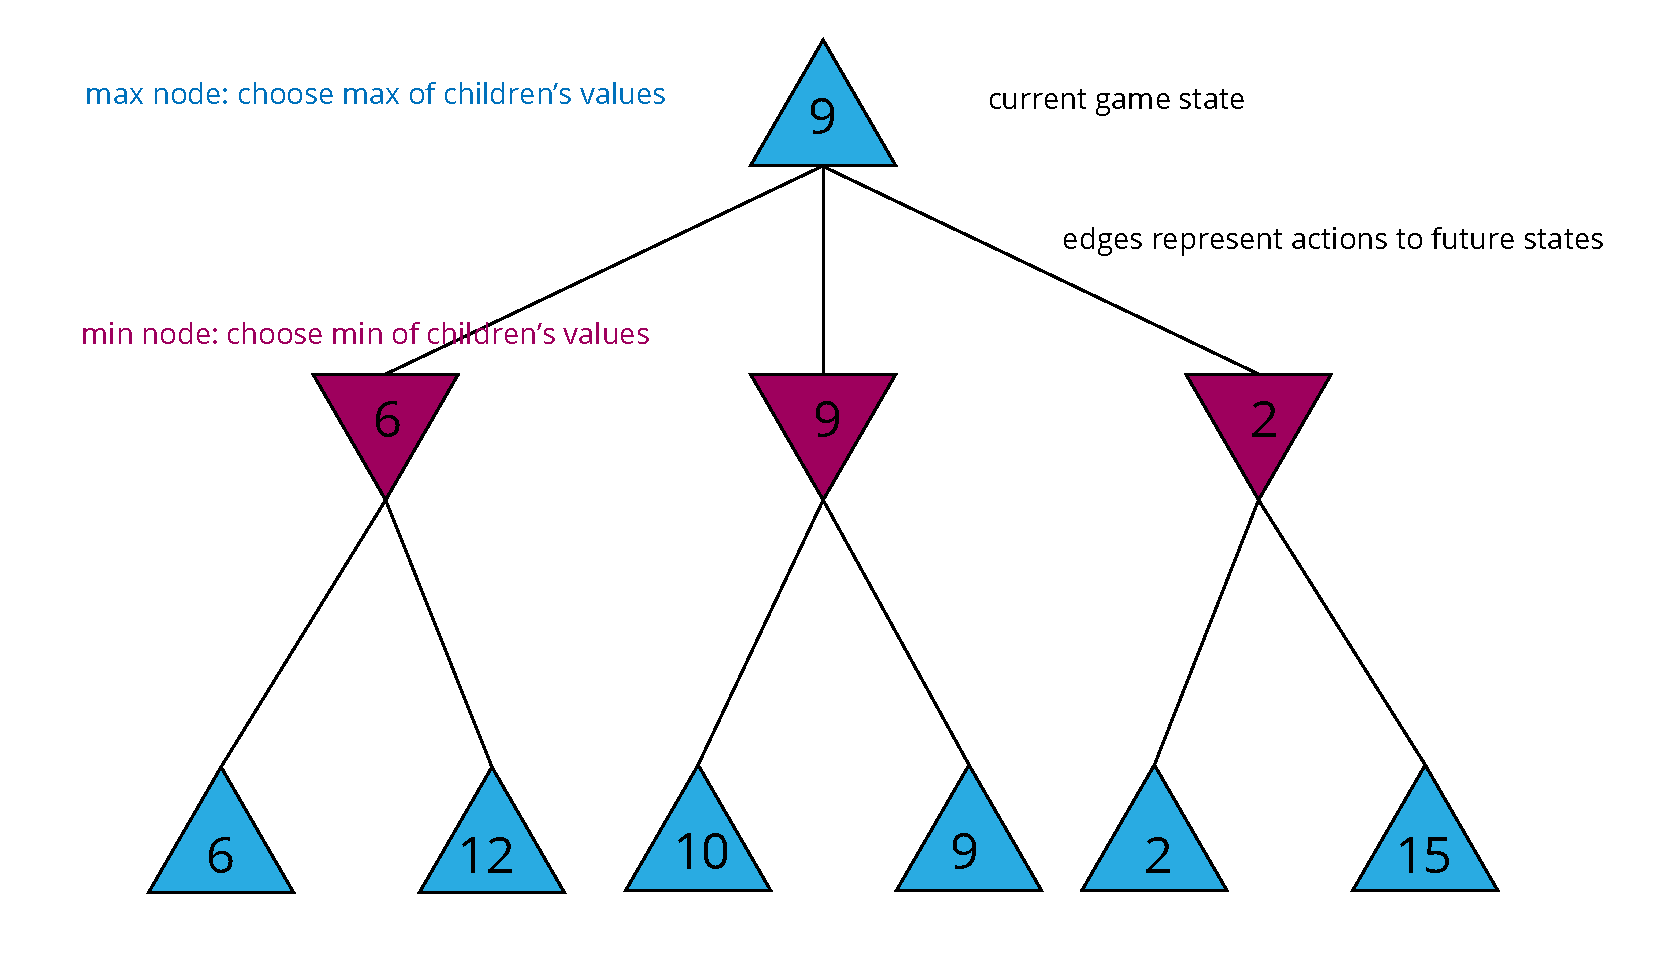
\includegraphics[scale=0.6]{minimaxtree.pdf}
\caption{{\bf Minimax Tree}}
\end{figure}

In the optimal scenario, the computer would be able to explore the minimax tree all the way down to its terminal nodes (nodes representing the end of the game). But for the game of chess, this is computationally infeasible towards the beginning of a game, due to the sheer number of possibilities that would have to be explored. Therefore, we must limit the depth of exploration to ensure that this search is tractable.

\section{Depth-Limited Minimax Implementation}

I implemented the minimax algorithm recursively. The processing of all nodes of the search tree with the exception of the root node is done with the functions \verb`maxValue` for max nodes and \verb`minValue` for min nodes in \verb`MinimaxAI.java`. Effectively, a depth-first search is done on the game tree and the max/min utility values of a node are determined as the recursion unwinds. Each node is passed a chess position to explore from, the current depth of exploration and the depth at which to cut off the search.

\vspace{5mm}

\begin{lstlisting}
private int maxValue(Position position, int depth, int cutoffDepth) {
  if (cutOffTest(position, depth, cutoffDepth)) {
    return utility(position);
  }
  int maxValue = - Integer.MAX_VALUE;
  short[] moves = position.getAllMoves();
  for (int i = 0; i < moves.length; i++) {
    short m = moves[i];
    try {
      position.doMove(m);
      maxValue = Math.max(maxValue, minValue(position, depth + 1, cutoffDepth));
      // Undo the move on original position so that we can try another
      position.undoMove();
    } catch(IllegalMoveException e) {
      System.out.println("Tried illegal move in minimax.");
    }
  }
  return maxValue;
}
\end{lstlisting}

\vspace{5mm}

\begin{lstlisting}
private int minValue(Position position, int depth, int cutoffDepth) {
  if (cutOffTest(position, depth, cutoffDepth)) {
    return utility(position);
  }
  int minValue = Integer.MAX_VALUE;
  short[] moves = position.getAllMoves();
  for (int i = 0; i < moves.length; i++) {
    short m = moves[i];
    try {
      position.doMove(m);
      minValue = Math.min(minValue, maxValue(position, depth + 1, cutoffDepth));
      // Undo the move on original position so that we can try another
      position.undoMove();
    } catch(IllegalMoveException e) {
      System.out.println("Tried illegal move in minimax.");
    }
  }
  return minValue;
}
\end{lstlisting}

\vspace{5mm}

If we reach a leaf node at a depth equal to the cutoff depth, we use the heuristic function \verb`utility` to evaluate the utility of the node. I first chose a rudimentary utility function that returns appropriate values for terminal states(high value for win, low value for loss, medium for stalemate) and a random value for everything else. An improvement to this heuristic will be discussed in the {\it Evaluation Functions} section.

\vspace{5mm}

\begin{lstlisting}
private int utility(Position position) {
  nodesExplored++;
  if (position.isTerminal()) {
    if (position.isMate()) {
      if (position.getToPlay() == this.color) {
        // I lose b/c opponent just checkmated me
        return - Integer.MAX_VALUE;
      } else {  // I win!
        return Integer.MAX_VALUE;
      }
    } else {  // no one wins
      return 0;
    }
  } else {
    return rand.nextInt(Integer.MAX_VALUE) - (Integer.MAX_VALUE / 2);
  }
}
\end{lstlisting}

\vspace{5mm}

The top-level function called from the current game state (root node) is a variation of \verb`maxValue` that, in addition to finding the highest utility child node found, tracks the move that leads to optimal path. 

\vspace{5mm}

\begin{lstlisting}
private void getMoveAtDepth(Position position, int cutoffDepth) {
  int value;
  short[] moves = position.getAllMoves();
  for (int i = 0; i < moves.length; i++) {
    short m = moves[i];
    try {
      position.doMove(m);
      value = minValue(position, 1, cutoffDepth);
      
      if (value > bestMoveValue) {
        bestMove = m;
        bestMoveValue = value;
      }
      position.undoMove();
    } catch(IllegalMoveException e) {
      System.out.println("Tried illegal move in minimax.");
    }
  }
}
\end{lstlisting}

\section{Iterative Deepening Minimax}

\subsection{Results: Finding Mate in 2}

\begin{figure}[!htb]
\centering

Average number of nodes explored in first 5 moves of game:
Depth 1: 57.8
Depth 2: 1769.4
Depth 3: 68628.6
Depth 4: 1086709.8
Depth 5: 32812052.4
Depth 6: 906909722.0

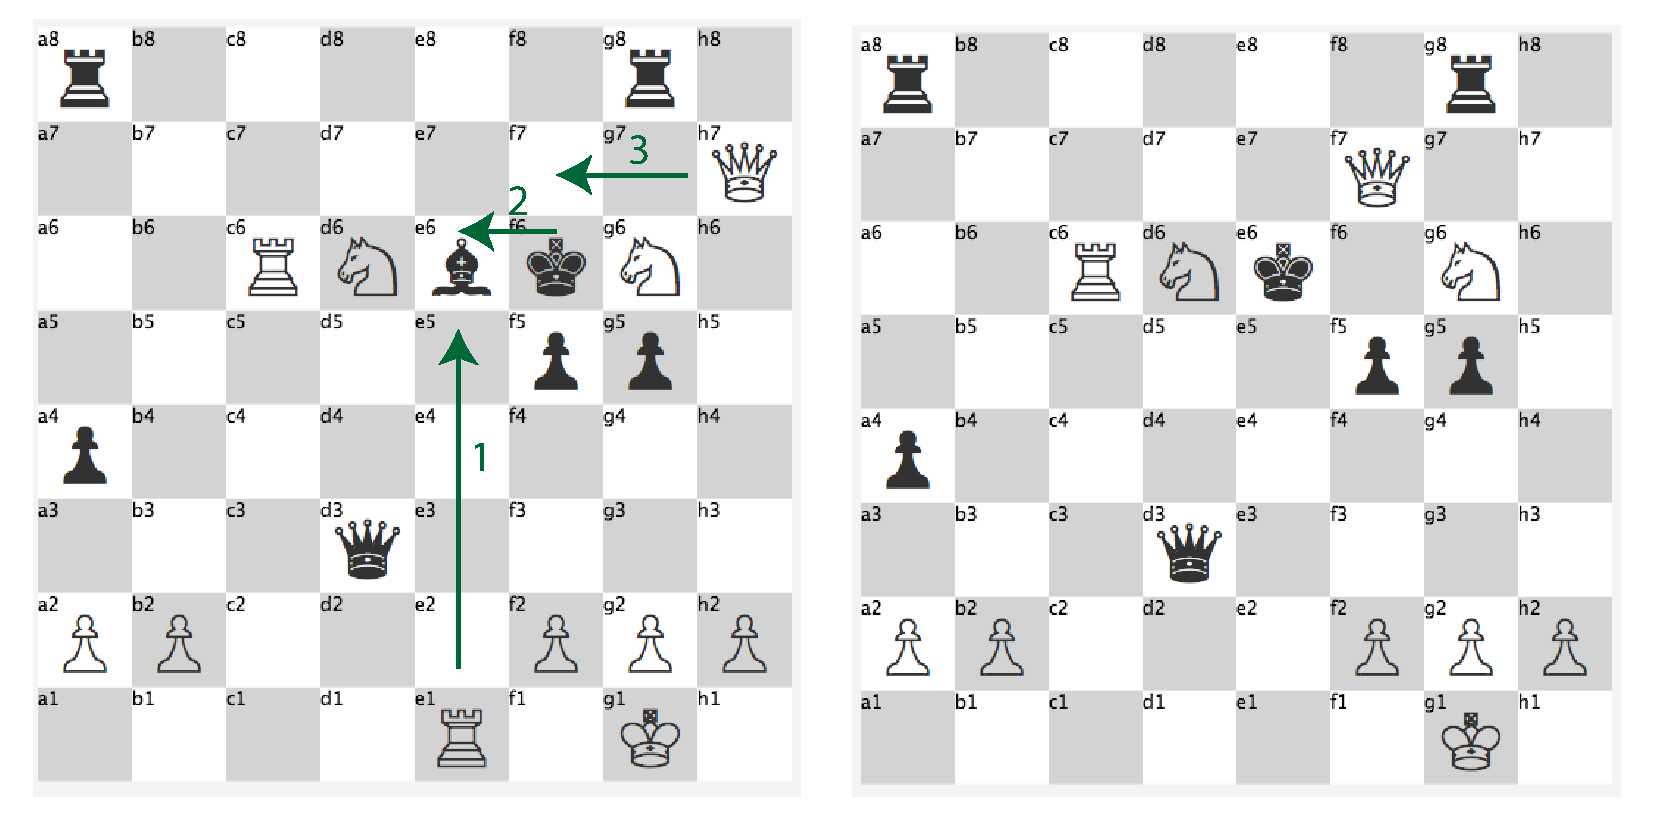
\includegraphics[scale=0.65]{mateintwo.pdf}
\caption{Mate in Two}
\end{figure}

Best move found at depth 1 has value 1072884021
Best move found at depth 2 has value 1072884021
Best move found at depth 3 has value 2147483647
Check!
Best move found at depth 1 has value 2147483647
Best move found at depth 2 has value 2147483647
Best move found at depth 3 has value 2147483647
Check!
Checkmate!

\section{Evaluation Functions}

\subsection{Material Utility}

\section{Alpha Beta Pruning}
While alpha-beta pruning does not improve the intrinsic "intelligence" of the AI, it allows for faster decisions to be made and exploration at deeper depths.

We can see the advantage of pruning by comparing the number of nodes explored in each move as an agent using minimax with alpha-beta pruning plays against an agent using minimax without alpha-beta pruning, both using iterative deepening search to a maximum depth of 6. Taking the average of the first 5 moves of the game, we find that using alpha-beta pruning clearly speeds up the efficiency of the search, as less nodes need to be explored.

Alpha Beta Nodes explored: 1007394
Minimax Nodes explored: 138769736
Alpha Beta Nodes explored: 2008097
Minimax Nodes explored: 393862788
Alpha Beta Nodes explored: 4371444
Minimax Nodes explored: 804099175
Alpha Beta Nodes explored: 8579693
Minimax Nodes explored: 1259678485
Alpha Beta Nodes explored: 12231582
Minimax Nodes explored: 1709415715
Alpha Beta Nodes explored: 17187151

\section{Transposition table}


\section{References}

Chess Programming Wiki. http://chessprogramming.wikispaces.com/

Marina Sirota, Francine Anene and Eric Mayefsky. "Strategies and Tactics for Intelligent Search". \\*http://www.stanford.edu/\textasciitilde msirota/soco.

\end{document}

